\documentclass[a4paper, 10pt]{article}
\usepackage[T1]{fontenc}
\usepackage[utf8]{inputenc}
\usepackage[slovene]{babel}
\usepackage{lmodern}
\usepackage{amsmath}
\usepackage{leftidx}
\usepackage{biblatex}
\usepackage{amssymb}
\usepackage{amsthm}
\usepackage{amsfonts}
\usepackage{graphicx}
\usepackage{wrapfig}
\usepackage{amsthm}
\usepackage{mathrsfs}
\usepackage{mathtools}
\usepackage{url}
\usepackage{subfigure}
\usepackage{multirow}
\usepackage{lipsum}
\usepackage{wrapfig}
\usepackage{tikz}
\usepackage[format=plain, font=small, labelfont=bf, textfont=it, justification=centerlast]{caption}
\usepackage{booktabs}
\usepackage{siunitx}

\newtheorem{izr}{Izrek}
\newtheorem{posl}{Posledica}[izr]

\newcounter{defcount}
\newcounter{opombe}
\newcounter{zgledcount}

\newenvironment{opomba}{\begin{flushleft}\stepcounter{opombe}\textbf{Opomba \arabic{opombe}:}}{\hfill\end{flushleft}}
\setlength{\parindent}{0mm}

\newenvironment{zgled}{\begin{flushleft}\stepcounter{zgledcount}\textbf{Zgled \arabic{zgledcount}:}}{\hfill\end{flushleft}}
\setlength{\parindent}{0mm}

\newenvironment{definicija}{\begin{flushleft}\stepcounter{defcount}\textbf{Definicija \arabic{defcount}:}}{\hfill\end{flushleft}}
\setlength{\parindent}{0mm}

\newcommand{\naslov}[1]{\textit{#1}}
\newcommand{\abs}[1]{\ensuremath{\lvert #1 \rvert}}
\newcommand{\mth}[1]{\ensuremath{\mathbb{#1}}}
\newcommand{\R}{\mth{R}}
\newcommand{\Z}{\mth{Z}}
\newcommand{\Zp}{\mth{Z}^{+}}
\newcommand{\N}{\mth{N}}
\newcommand{\No}{\mth{N}_0}
\newcommand{\C}{\mth{C}}
\newcommand{\Qu}{\mth{Q}_u}
\newcommand{\pojem}[1]{\emph{#1}}
\newcommand{\con}{\ensuremath{\mathscr{C}}}
\newcommand{\padex}[2]{\ensuremath{{#1}^{\underline{#2}}}}
\newcommand{\rastx}[2]{\ensuremath{{#1}^{\bar{#2}}}}
\newcommand{\map}[3]{\ensuremath{{#1}: {#2} \rightarrow {#3}}}
\newcommand{\pra}[3]{{#1}{\ast}({#2}) = {#3}}

\title{Projektna naloga pri Statistiki}
\date{17.7.2022}
\author{Jimmy Zakeršnik}
%===============================================================================
\begin{document}
	\maketitle
	\thispagestyle{empty}
	\newpage
	\begin{abstract}
		V tej projektni nalogi pri predmetu Statistika, bom obravnaval tri naloge po navodilih. Vsaka naloga bo obravnavana v svojem lastnem poglavju. Da bo se lažje sklicevati na njih, bo prva naloga poimenovana \pojem{Kibergrad}, druga \pojem{Slučajni sprehod} in tretja \pojem{Temperature}.
	\end{abstract}
	\newpage
	\tableofcontents
	\newpage
	\section{Kibergrad}\label{sect: Kibergrad}
	Priložena datoteka \textit{Kibergrad.csv}, ki vsebuje podatke o dani populaciji (prebivalci mesta Kibergrad), je bila odprta v programu LibreOffice Calc. S pomočjo vgrajenega orodja so nato, bili zbrani vzorci velikosti $500$ po postopku enostavnega vzorčenja. V priloženi datoteki \textit{Kibergradwork.ods} so na prvi strani izpisani vsi podatki ter vseh pet pridobljenih vzorcev, na drugi strani je posebej obravnavan prvi vzorec v smislu kvartilov in extremnih vrednosti, na tretji strani pa se na enak način obravnavajo vsi vzorci glede na dohodek družin tipa $1$. Obe primerjavi sta dodatno podprti s pomočjo škatel z brki in na koncu sta izračunani še s tipi pojasnjena varianca in nepojasnjena varianca dohodkov. Pri tem je v veliko pomoč programski jezik R.
	
	\subsection{Primerjava dohodkov med tipi družin prvega vzorca} \label{subsect: 1A}
	Poglejmo si najprej prvi vzorec in primerjajmo dohodke družin glede na tip družine. V delovnem okolju jezika $\textbf{R}$ odpremo in poženemo skripto \textit{Kibergrad\_a.R}. Ob pogonu se v konzoli izpišejo vrednosti o dohodku, ki so navedene v spodnji tabeli.
	\begin{table}[h!]
		\label{tab: quartA}
		\centering
		\begin{tabular}{|l|c|c|c|}
			\hline
			& Tip $1$ & Tip $2$ & Tip $3$ \\ \hline
			Max & $228727$ & $181696$ & $168926$ \\ \hline
			Q$3$ & $55360$ & $54859$ & $57631$ \\ \hline
			Med & $32975$ & $38883$ & $33310$ \\ \hline
			Q$1$ & $18700$ & $22011$ & $16071$ \\ \hline
			Min & $0$ & $5184$ & $0$ \\ \hline
		\end{tabular}
	\caption{Tabela vrednosti, ki so potrebne za risanje škatel z brki za vsak tip družine}
	\end{table}

	Istočasno skripta izriše vzporedne škatle z brki, kot lahko vidimo na spodnji sliki, s pomočjo katerih lahko grafično primerjamo dohodke družin različnih tipov.
	
	\begin{figure}[h!]
		\label{fig: boxplotA}
		\centering
		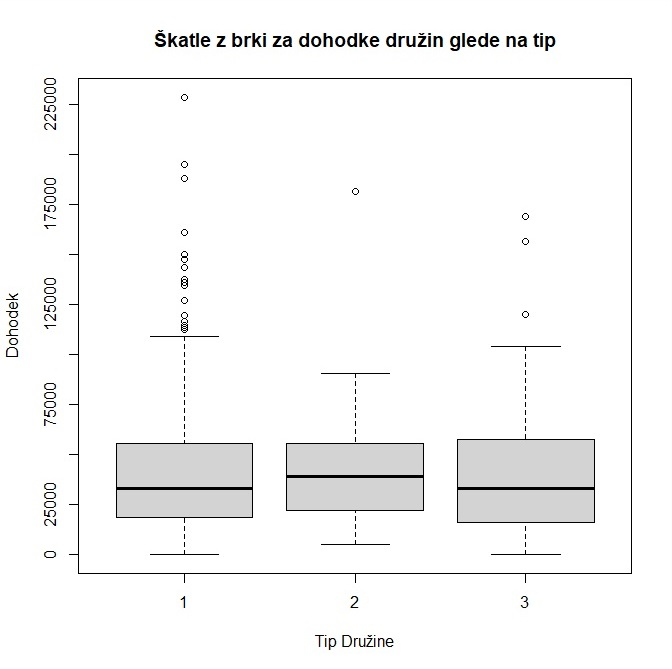
\includegraphics[scale = 0.35]{TabelaSample1}
		\caption{Vzporedno narisane škatle z brki tipov družin $1$, $2$ in $3$}
	\end{figure}
%	\newpage
	Škatle z brki nam ponudijo nekaj zanimivih ugotovitev. V minimalnih dohodkih ni velikih odstopanj, razen pri tipu $2$, ki ima za razliko od ostalih pozitiven minimalen dohodek. Če ignoriramo ostale vzorce in tem rezultatom naivno verjamemo, so enostarševske družine z očetom (torej družine tipa $2$) relativno bolj premožne od ostalih tipov. To domnevo podpira tudi opazka, da je povprečna vrednost tipa $2$ višja kot povprečni vrednosti ostalih dveh tipov, kar lahko preberemo iz izpisa na konzoli. 

	Vrednosti so hkrati tudi dostopne v spodnji tabeli. 

	\begin{table}[h!]
		\label{tab: MeanSDA}
		\centering
		\begin{tabular}{|l|c|c|c|}
			\hline
			Tip & $1$ & $2$ & $3$ \\ \hline
			Povprečje & $41655$ & $46301$ & $39931$ \\ \hline
			SD & $32974{,}23$ & $39500{,}3$ & $31069{,}71$ \\ \hline
		\end{tabular}
	\caption{Povprečne vrednosti in standardni odkloni dohodkov po tipih}
	\end{table}

	Če ne bi imeli že izračunanih povprečij, bi lahko še vedno sklepali o njihovih velikostih s pomoćjo škatel z brki. Opazimo namreč, da se prvi kvartili nahajajo na približno enaki višini z maksimalno razliko v okolici $6000$ v prid družinam tipa $2$, kar velja tudi za mediane. Šele pri tretjem kvartilu ostala dva tipa premagata tip $2$, a tudi tu je največja razlika v rangu $4000$. V tem primeru tipu $2$ pomaga to, da ima izmed vseh tipov družin najmanjšo razdaljo med tretjim kvartilom in mediano, kar pomeni, da so vrednosti, ki pripadajo temu intervalu, bolj gosto porazdeljene.

	Višje povprečje dohodka družin tipa $2$ ni edino, kar izstopa pri škatlah z brki. Družine tipa $1$ izstopajo v tem, da imajo, v primerjavi z ostalimi tipi, veliko število osamelcev (torej tistih vrednosti, ki so na sliki označene s krogi izven škatel).

	Družine tipa $3$ se odlikujejo po tem, da imajo najširši interkvartilni razmik. Za lažji pregled in primerjavo, so vsi interkvartilni razmiki navedeni v konzoli (po pogonu skripte) ter v tabeli spodaj:
	\begin{table}[h!]
		\label{tab: IQRA}
		\centering
		\begin{tabular}{|l|c|c|c|}
			\hline
			Tip & $1$ & $2$ & $3$ \\ \hline
			IQR & $36660$ & $32848$ & $41560$ \\ \hline
		\end{tabular}
		\caption{Interkvartilni razmiki dohodkov po tipih}
	\end{table}

	Družine tipa $2$ so torej v povprečju bolj premožne od družin ostalih tipov in družine tipa $3$ so v povprečju najmanj premožne. Vrednosti družin tipa $3$ so hkrati tudi najbolj razpršene v >>srednji polovici<<, kar nam pove velikost interkvartilnega razmika. Družine tipa $1$ se v obeh primerih nahajajo v sredini med družinami tipa $2$ in $3$. Hkrati imajo tudi razmeroma več osamelcev od ostalih tipov. V vsakem primeru nam rezultati namigujejo, da obstaja povezava med tipom družine in njenim dohodkom.
	\newpage
	\subsection{Primerjava dohodkov družin tipa $1$ v petih vzorcih}\label{subsect: 1B}
	Da nadaljujemo analizo podatkov si oglejmo porazdelitev dohodkov družin nekega tipa preko 5 neodvisno izbranih vzorcev. Pri tem za prvega vzamemo kar vzorec, ki smo ga obravnavali v prejšnjem podpoglavju, ostale štiri pa pridobimo s pomočjo orodij v LibreOffice Calc. Vsi vzorci so posebej shranjeni v lastni datoteki tipa \textit{.csv} z imeni tipa \textit{KibergradVzorec$\#$.csv}.

	Da izrišemo škatle z brki, s pomočjo katerih bomo primerjali dohodke preko vzorcev, poženemo skripto \textit{Kibergrad\_b.R}. V njej najprej naložimo vzorce, nato vsakemu vzorcu dodamo stolpec vrednosti, ki nam pove kateremu vzorcu pripada dan podatek. Torej vzorcu $1$ dodamo stolpec samih enk, vzorcu $2$ stolpec samih dvojk itd. Te tabele nato združimo v eno samo tabelo, iz nje prefiltriramo družine vseh tipov razen $1$ in nato s pomočjo te nove tabele po enakem postopku kot v prejšnjem podpoglavju primerjamo dohodke družin glede na vzorec.

	Dobljene škatle z brki so prikazane spodaj.

	\begin{figure}[h!]
		\label{fig: boxplotB1}
		\centering
		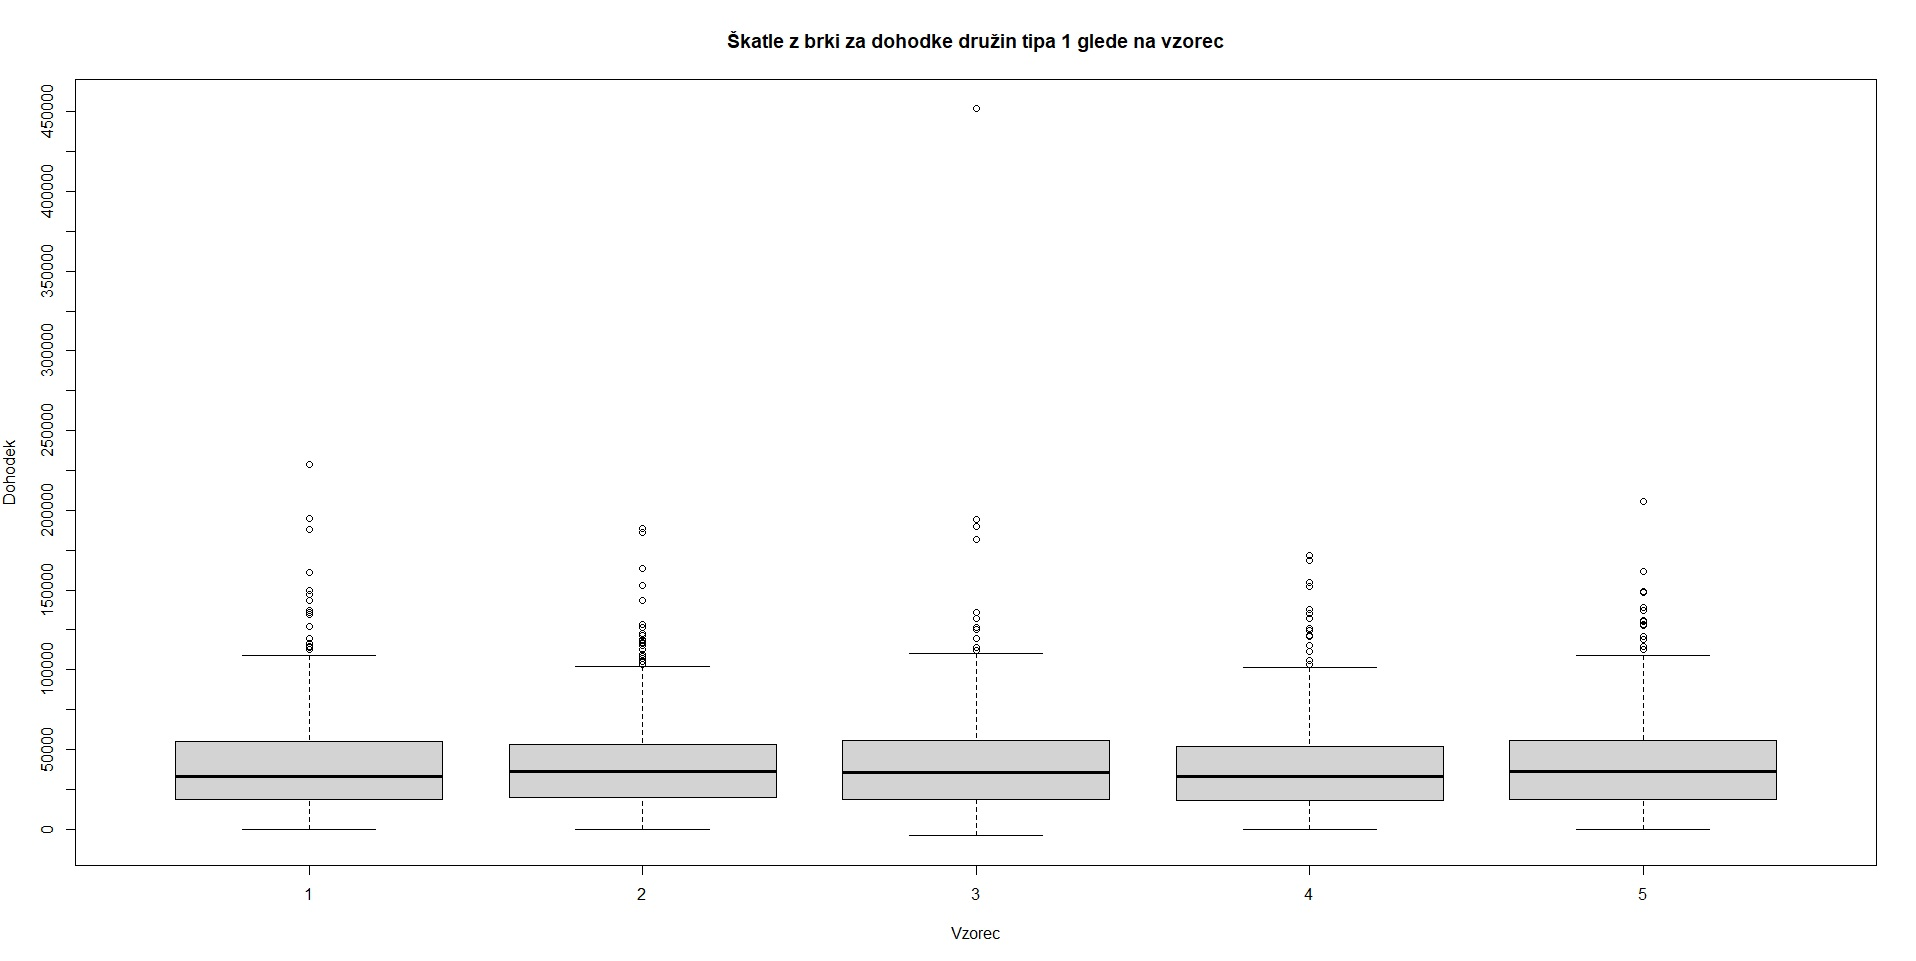
\includegraphics[scale = 0.425]{SkatlezbrkiB}
		\caption{Vzporedno narisane škatle z brki družin tipa $1$ po vzorcih}
	\end{figure}

	Takoj opazimo, da je prikazan graf razpotegnjen, v glavnem na račun enega osamelca iz tretjega vzorca. Da dobimo bolj pregleden graf, odstranimo vse vrednosti, ki so večje od $250000$ (v resnici je taka zgolj ena). Škatle z brki, ki jih dobimo po tem popravku in so prikazane spodaj, skripta samostojno izriše.
	\newpage
	\begin{figure}[h!]
		\label{fig: boxplotB2}
		\centering
		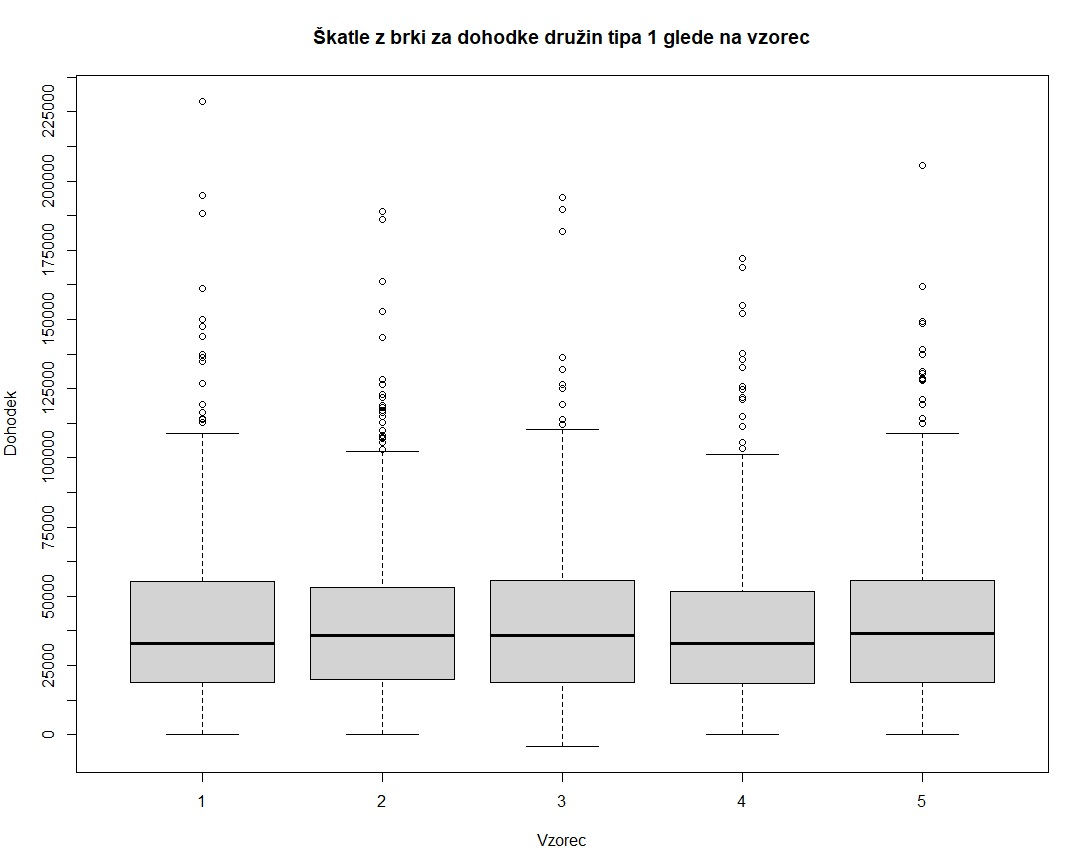
\includegraphics[scale = 0.4]{LepseSkatlezbrkiB}
		\caption{Popravljene vzporedno narisane škatle z brki družin tipa $1$ po vzorcih}
	\end{figure}
	
	Ker smo pri >>popravku<< zanemarili zgolj eno vrednost, nam to bistveno ne pokvari primerjave. Izoliran osamelec bi lahko na našo obravnavo vplival kvečjemu negativno. Zato bomo pri izračunu povprečja za vsak vzorec uporabili tabelo, ki tega osamelca ne vsebuje.
	
	Vrednosti (kvartili, povprečja, maksimalna in minimalna vrednost, IQR), ki jih skripta izpiše v konzolo, so prikazane v spodnji tabeli:
	
	\begin{table}[h!]
		\label{tab: QuartMeanA}
		\centering
		\begin{tabular}{|l|c|c|c|c|c|}
			\hline
			 & Vzorec $1$ & Vzorec $2$ & Vzorec $3$ & Vzorec $4$ & Vzorec $5$ \\ \hline
			Max & $228727$ & $188899$ & $194230$ & $171999$ & $205712$ \\ \hline
			Q$3$ & $55360$ & $53121$ & $55700$ & $51700$ & $55863$ \\ \hline
			Med & $32975$ & $36000$ & $35850$ & $33006$ & $36527$ \\ \hline
			Q$1$ & $18700$ & $20008$ & $18800$ & $18327$ & $18668$ \\ \hline
			Min & $0$ & $0$ & $-4198$ & $0$ & $0$ \\ \hline
			\hline
			Povprečje & $41655$ & $41822$ & $41337$ & $39344$ & $41697$ \\ \hline
			SD & $32974{,}23$ & $31037{,}97$ & $30517{,}25$ & $29867{,}4$ & $31099{,}04$ \\ \hline
			IQR & $36660$ & $33113$ & $36900$ & $33373$ & $37195$ \\ \hline
		\end{tabular}
		\caption{Ekstremi, kvartili, povprečja, standardni odkloni in interkvartilni razmiki dohodkov družin tipa $1$ po vzorcih}
	\end{table}
	
	Sedaj, ko imamo narisane škatle z brki in zraven napisano tabelo, lahko komentiramo rezultate. V prvi vrsti opazimo, da so si povprečja dokaj blizu. Vsa povprečja razen povprečje četrtega vzorca se nahajajo v okolici $41500 \pm 500$, povprečje vzorca $4$ pa se od $41500$ razlikuje za manj kot $2500$. Če bi si izbrali še već vzorcev, bi se po vsej verjetnosti njihova povprečja tudi nahajala v neki bližnji okolici $41500$. Podobno obnašanje standardnih odklonov, ki se nabirajo v okolici $31000 \pm 2000$ nas privede do nepresenetljivega sklepa, da je dohodek družin tipa $1$ porazdeljen po vzorcih, torej porazdelitev dohodka ni odvisna od vzorca. To potrjuje tudi relativna bližina kvartilov v tabeli (npr. tretji kvartili se zbirajo v okolici $53000 \pm 3000$).
	
	Na tej točki bi želeli preveriti, ali je porazdelitev slučajno normalna. Tako test s primerjalnim kvartilnim grafikonom kot Shapiro-Wilkov test na vzorcu $1$ nam poveta, da to ne drži. V primeru Shapiro-Wilkovega testa, dobimo vrednost $p < 2.2e{-16} < 0.05$, torej porazdelitev ni normalna. To vidimo tudi na primerjanlen kvartilnem grafikonu spodaj. Enak sklep seveda velja tudi za ostale vzorce.
	
	\begin{figure}[h!]
		\label{fig: qqplotB}
		\centering
		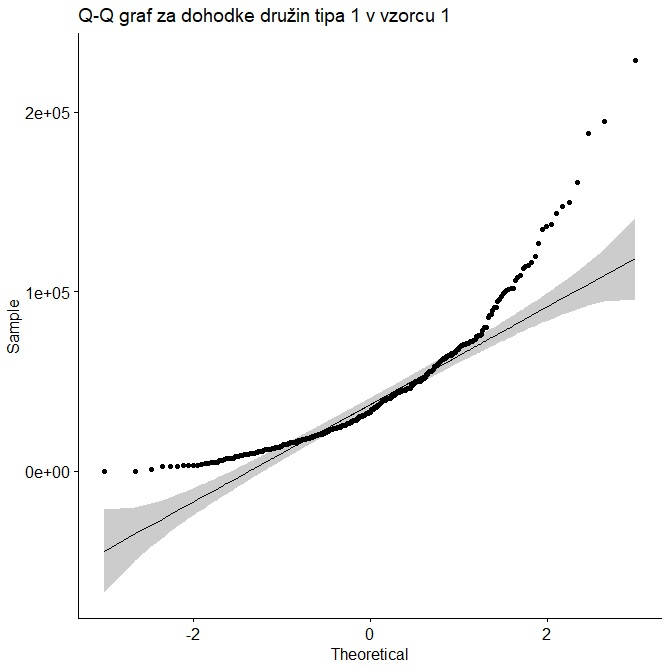
\includegraphics[scale = 0.5]{QQVzorec1}
		\caption{Primerjalni kvartilni grafikon dohodkov družin tipa $1$ v vzorcu 1}
	\end{figure}
	
	Četudi dohodki niso porazdeljeni normalno, so še vedno razmeroma konsistentni preko obravnavanih vzorcev. To je v kontrastu z razlikami in odstopanji, ki smo jih opazili, ko smo v prvem vzorcu primerjali dohodke glede na tip družine. Ta kontrast dodatno potrjuje sklep, da tip družine netrivialno vpliva na dohodek družine. 
	
	\subsection{S tipom pojasnjena varianca populacije}\label{subsect: 1C}
	Na koncu prejšnjega podpoglavja smo prišli do sklepa, da ima tip družine netrivialen vpliv na dohodek družine. Če to drži ali ne, lahko preverimo z izračunom s tipom družine pojesnjene variance. Čim smo poračunali to, se lahko skličemo na zvezo med varianco in pojasnjeno ter nepojasnjeno varianco ($Celotna\_varianca = Pojasnjena\_varianca + Nepojasnjena\_varianca$) in poračunamo še slednjo. Vsi računi in primerjave se prikažejo ob pogonu skripte \textit{Kibergrad\_c.R}. 
	
	Z $n_i$ označimo število družin tipa $i$ ter z $N$ velikost naše populacije. Z $X$ označimo dohodke družin, z $Y$ pa  slučajno spremenljivko tipov družin, ki ima porazdelitev $P(Y = i) = n_i / N$. Predpostavimo, da so dohodki tipov družin $X_i = X_{|Y=i}$ medseboj neodvisni. Predpostavko upravičimo z argumentom, da v splošnem dohodek soseda ne vpliva na naš dohodek. Pomnimo tudi, da je $E\left[X|Y\right]$ neka funkcija spremenljivke $Y$, recimo $\Phi(Y)$.
	Z $\bar{X}_i$ še označimo pričakovano vrednost dohodka v družini tipa $i$, torej $\bar{X}_i = E\left[X|Y = i\right]$. S tipom pojasnjeno varianco potem izračunamo po formuli: 
	\begin{align*} \label{eq: explvarC}
		& Var(E\left[X|Y\right]) = Var(\Phi(Y)) = E\left[(\Phi(Y)- E\left[\Phi(Y)\right])^2\right] =\\ 
		&= \sum_{i = 1}^{3} (\Phi(Y = i)- E\left[\Phi(Y)\right])^2 * P(Y = i) = 1/N * \sum_{i = 1}^{3} n_i * (E\left[X|Y = i\right] - E\left[E\left[X|Y\right]\right])^2 \\ &= 1/N * \sum_{i = 1}^{3} n_i * (\bar{X}_i - E\left[X\right])^2 = 1/N * \sum_{i = 1}^{3} n_i * (\bar{X}_i - \bar{X})^2
	\end{align*}

	S pomočjo zgoraj pridobljene formule v \textit{Kibergrad\_c.R} poračunamo pojasnjeno varianco. Nepojasnjeno varianco nato poračunamo kot razliko populacijske variance in pojasnjene variance. Vrednosti skripta izpiše v konzolo, dostopne pa so tudi v spodnji tabeli.
	
	\begin{table}[h!]
		\label{tab: varC}
		\centering
		\begin{tabular}{|l|c|}
			\hline
			Varianca & $1026385670$ \\ \hline
			Pojasnjena & $113781162$ \\ \hline
			Nepojasnjena & $912604508$ \\ \hline
			SD & $32037{,}2544062437$ \\ \hline
		\end{tabular}
		\caption{Populacijska, s tipi pojasnjena in nepojasnjena varianca}
	\end{table}
	
	Opazimo, da je nepojasnjena varianca bistveno višja od pojasnjene variance. Če pogledamo delež, ki ga varianci zavzemata, nam s tipi družin pojasnjena varianca predstavlja le približno $11{,}09\%$. To nam pove, da je tip družine netrivialen faktor pri napovedi dohodka družine, ni pa glavni faktor. To se ujema s tem, kar smo razbrali v prejšnjih podpoglavjih. Že zgolj za družine tipa $1$ v podpoglavju \ref{Subsect: 1B} je bil standardni odklon, torej koren variance, razmeroma visok v vsakem vzorcu. To se ujema s tem, da večino variance pridobimo od faktorjev, ki niso tip družine. Če bi tip družine bil odgovoren za večji delež celotne variance dohodkov, bi bila varianca znotaj tipov manjša.
	
	\section{Slučajni sprehod} \label{sect: SlucajniSprehod}
	
	\subsection{Cenilka za $\theta$ po metodi največjega verjetja} \label{subsect: 2A}
	
	\subsection{Cenilka za $\theta$ po metodi momentov}\label{subsect: 2B}
	
	\subsection{Asimptotični $MSE$ cenilk}\label{subsect: 2C}
	
	\subsection{Številska ocena prve cenilke} \label{subsect: 2D}
	
	\subsection{Številska ocena druge cenilke} \label{subsect: 2E}
	
	\subsection{Histogram meritev in grafi gostot cenilk} \label{subsect: 2F}
	
	\section{Temperature}\label{sect: Temperature}
	
	\subsection{Preizkus modela $A$ znotraj modela $B$}\label{susect: 3A}
	
	\subsection{Akikakejeva informacija modelov}\label{subsect: 3B}
	
	
\end{document}